\section{Network}

For one neuron there is one output value so we can easily see that one is not enough to solve many problems. Combining neurons into networks and layers will make them more useful. But one single neuron is still able to solve some class of problems.

\begin{wrapfigure}{r}{0.3\textwidth}
    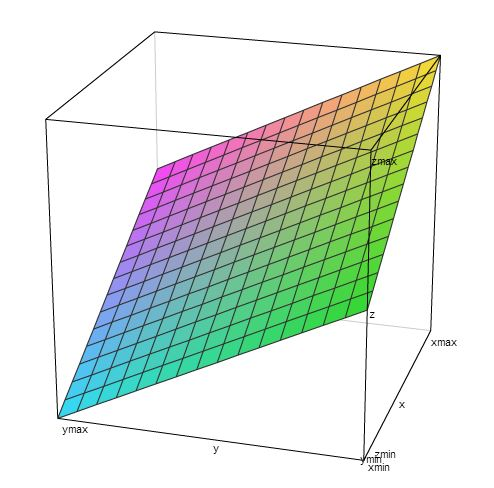
\includegraphics[width=0.32\textwidth]{Media/Plane.png}
    \caption{Single neuron plane}
    \label{fig:Plane}
\end{wrapfigure}

Typically each neuron has one constant input value. If we try to show graphical interpretation of neuron it will become clear why and also what class of problems can be solve with one neuron only.

Consider a neuron with two inputs $n = 2$ and with random weights $w_n$. So we have three axis, two for input data and one to show neuron output.

Without one constant input graph of such neuron would be just a random set of points in 3D space. But if we set one of the inputs constant we will obtain a 3D plane.




\subsection{Layers}

\subsection{MLNN/PLP}

\subsection{Training}